\documentclass[a4paper,12pt]{report}
\usepackage[utf8]{inputenc}
\usepackage{multicol}
\usepackage[T1]{fontenc}
\usepackage[top=0.8in,bottom=1in,right=1in,left=1in]{geometry}
\usepackage{graphicx}
\usepackage{color}
\usepackage{listings}
\usepackage{fancyhdr}
\usepackage{xcolor}
\usepackage{ebgaramond}
\usepackage{minitoc}
\usepackage[skip=2pt,labelfont=bf]{caption}
\definecolor{one}{RGB}{90,0,0}
\definecolor{two}{RGB}{0,0,70}
\definecolor{three}{RGB}{88,68,68}


\lstdefinestyle{mystyle}{
	language=python,
    commentstyle=\color{three},
    keywordstyle=\color{two},
    numberstyle=\footnotesize\color{one},
    stringstyle=\color{three},
    basicstyle=\ttfamily\sf,
    breakatwhitespace=false,         
    breaklines=true,                 
    captionpos=b,                    
    keepspaces=true,                 
    numbers=left,                    
    numbersep=5pt,                  
    showspaces=false,                
    showstringspaces=false,
    showtabs=false,                  
    tabsize=2
}
\lstset{style=mystyle}
\begin{document}
\pagestyle{fancy}
\fancyhf{}
\rhead{\textit{\textsf{\leftmark}}}
\cfoot{\thepage}
\begin{center}
		\Large{A Training Report On}\\[0.5cm]
		\underline{\color{two}\textbf{\Large{Data Structures and Algorithms in Python}}}\\[1cm]

		\Large{Submitted in partial fulfillment of the
		requirements}\\[0.1cm]
		\Large{For The Degree Of }\\[0.1cm]
		\textbf{\large{BACHELOR OF TECHNOLOGY}}\\[0.1cm]
		\Large{in}\\[0.1cm]
		\textbf{\large{ELECTRONICS AND COMMUNICATION
		ENGINEERING}}\\[0.7cm]
\end{center}
\begin{center}
\includegraphics[scale=0.24]{"ctae.jpg"}\\[0.5cm]
		\textbf{Session 2019-2020}\\
		\rule{3cm}{0.3mm}\\[1mm]
		\textbf{Training Duration (from 3/5/20 to 27/5/20)}\\[1.8cm]
\end{center}
\begin{multicols}{2}
	\begin{flushleft}
		\large{\textbf{Submitted to}}\\
		\large{\textrm{Navneet}}\\[0.4cm]
		\large{\textbf{Enrollment No.}}\\
	\end{flushleft}
	\begin{flushright}
		\large{\textbf{Submitted by}}\\
		\textrm{Navneet}\\[0.4cm]
		\large{\textbf{Subject Code}}\\
	\end{flushright}
\end{multicols}
\vspace{1.5cm}
\textbf{III year ECE}\\[0.5cm]
\rule{\textwidth}{0.3mm}
\begin{center}
	\textbf{DEPARTMENT OF ELECTRONICS AND COMMUNICATION ENGINEERING}\\[0.0cm]
	\large{\color{black}\textbf{COLLEGE OF TECHNOLOGY AND ENGINEERING}}\\
	\textbf{\scriptsize{MAHARANA PRATAP UNIVERSITY OF AGRICULTURE AND
	TECHNOLOGY,UDAIPUR,RAJASTHAN}}
	\rule{\textwidth}{0.3mm}\\[0.19cm]
	\color{three}\textbf{Compiled in \LaTeX}
\end{center}
\thispagestyle{empty}
\begin{center}
\thispagestyle{empty}
	\textbf{ }\\[5cm]
\textbf{\LARGE{Certificate}}\\
\begin{figure}[h]
	
\includegraphics[scale=0.3]{udemy.jpg}
\end{figure}
\end{center}
	\rule{16cm}{0.5mm}\\[8.3cm]
	\begin{center}
		\textrm{(i)}
	\end{center}
\newpage

\begin{center}
\thispagestyle{empty}
	\textbf{ } \\[4cm]
	\textbf{\LARGE{Acknowlegement}}\\[1cm]
	\Large{I would like to express my special thanks of gratitude to my teacher
	\textbf{Dr.Navneet Agarwal & Dr.Sunil Joshi} as well as our principal (Name of the principal)who gave me the golden opportunity to do this wonderful project on the topic (Write the topic name), which also helped me in doing a lot of Research and i came to know about so many new things I am really thankful to them.
Secondly i would also like to thank my parents and friends who helped me a lot
	in finalizing this project within the limited time frame.}
\end{center}


\dominitoc \tableofcontents
\listoffigures
\newgeometry{top=1in,bottom=1.15in,left=1.5in,right=0.6in}
\chapter{Analysing Time Complexity}
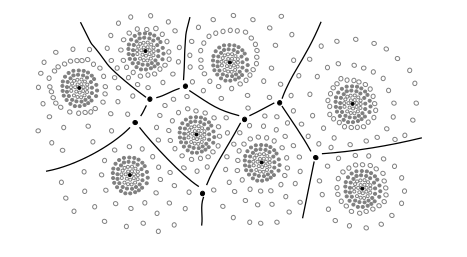
\includegraphics[scale=0.9]{babu.png}
\minitoc
\newpage
\section{Introduction}
Algorithmic complexity is concerned about how fast or slow particular algorithm
performs. We define complexity as a numerical function $T(n)$ - time versus the
input size $n$. We want to define time taken by an algorithm without depending
on the implementation details. But you agree that $T(n)$ does depend on the
implementation! A given algorithm will take different amounts of time on the
same inputs depending on such factors as: processor speed; instruction set,
disk speed, brand of compiler and etc. The way around is to estimate efficiency
of each algorithm asymptotically. We will measure time $T(n)$ as the number of elementary "steps" (defined in any way), provided each such step takes constant time. 
\\[0.4cm]

Let us consider two classical examples: addition of two integers. We will add
two integers digit by digit (or bit by bit), and this will define a "step" in
our computational model. Therefore, we say that addition of two n-bit integers
takes n steps. Consequently, the total computational time is $T(n) = c * n$,
where c is time taken by addition of two bits. On different computers, additon
of two bits might take different time, say c1 and c2, thus the additon of two
n-bit integers takes $T(n) = c1 * n$ and $T(n) = c2 * n$ respectively. This
shows that different machines result in different slopes, but time $T(n)$ grows linearly as input size increases.
\begin{figure}[h]
	\begin{center}
	\includegraphics[scale=0.5]{"fig1.png"}
	\end{center}
	\caption{\textsf{Results of an experimental study on the running time of an algorithm.
	A dot with coordinates $(n,t)$ indicates that on an input of size $n$, the running time
	of the algorithm was measured as $t$ milliseconds (ms).}}
\end{figure}
\section{Counting Primitive Operations}
To analyze the running time of an algorithm without performing experiments, we
perform an analysis directly on a high-level description of the algorithm (either in
the form of an actual code fragment, or language-independent pseudo-code). We
define a set of \textit{\textbf{primitive operations}} such as the following:
\begin{itemize}
	\item Assigning an identifier$^1$ to an object
	\item Determining the object associated with an identifier
	\item Performing an arithmetic operation (for example, adding two numbers)
	\item Comparing two numbers
	\item Accessing a single element of a Python list by index
	\item Calling a function (excluding operations executed within the function)
	\item Returning from a function.
\end{itemize}
An algorithm may run faster on some inputs than it does on others of the same size.
Thus, we may wish to express the running time of an algorithm as the function of
the input size obtained by taking the average over all possible inputs of the same
size. Unfortunately, such an average-case analysis is typically quite challenging.
It requires us to define a probability distribution on the set of inputs, which is often
a difficult task. \textbf{Figure} \ref{fig2} schematically shows how, depending on the input distribution, the running time of an algorithm can be anywhere between the worst-case
time and the best-case time. For example, what if inputs are really only of types
“A” or “D”?
\begin{figure}[h]
	\label{fig2}
	\centering
	\includegraphics[scale=0.65]{"fig2.png"}
	\caption{\label{fig2}\textsf{ The difference between best-case and worst-case time.
	Each bar represents the running time of some algorithm on a different
	possible input.}}
\end{figure}
\footnote{Python's identifier is similar to Reference varible in Java or
pointer variable in C++}
\\
An average-case analysis usually requires that we calculate expected running
times based on a given input distribution, which usually involves sophisticated
probability theory.We will characterize running times in terms of the \textit{\textbf{worst
case}}, as a function of the input size, n, of the algorithm.\\
If an algorithm has been implemented, we can study its running time by executing
it on various test inputs and recording the time spent during each execution. A
simple approach for doing this in Python is by using the time function of the time
module. This function reports the number of seconds, or fractions thereof, that have
elapsed since a benchmark time known as the epoch. The choice of the epoch is
not significant to our goal, as we can determine the elapsed time by recording the
time just before the algorithm and the time just after the algorithm, and computing
their difference, as follows:\\
\begin{lstlisting}[language=Python,caption=\textsf{Calculating Run time}]
! /run/media/mukul/D/SH/test.py
from time import time
start time = time()  		# record starting time
num=[1,2,-2,5,6,6]
target=3
for i in range(len(num)): #Two Sum
    x=num[i]
    for j in range(i+1,len(num)):
        if num[j]==target-x:
            print(i,j)
end time = time()		# record ending time
elapsed = end_time - start_time # compute the elapsed time
\end{lstlisting}
\begin{figure}[h]
	\centering
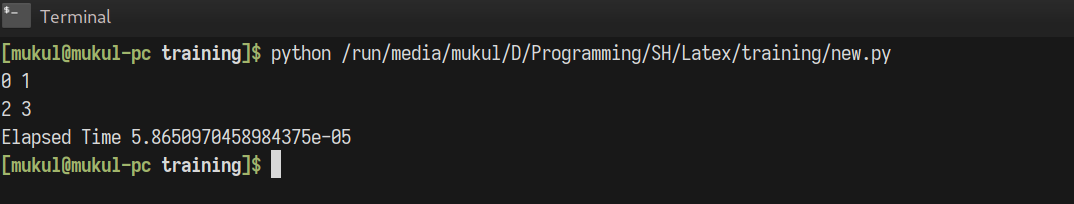
\includegraphics[scale=0.45]{piku.png}
	\caption{Output of Listing 1.1}
\end{figure}
\section{Functions used in Analysis of Algorithms}
\newpage





\chapter{Stacks}
\newpage
\section{Introduction}
A \textbf{\textit{stack}} is a collection of objects that are inserted and removed according to the
\textbf{last-in, first-out (LIFO) principle}. A user may insert objects into a stack at any
time, but may only access or remove the most recently inserted object that remains
(at the so-called “top” of the stack). The name “stack” is derived from the metaphor
of a stack of plates in a spring-loaded, cafeteria plate dispenser. In this case, the
fundamental operations involve the “pushing” and “popping” of plates on the stack.
When we need a new plate from the dispenser, we “pop” the top plate off the stack,
and when we add a plate, we “push” it down on the stack to become the new top
\section{Basic Functions that Stack supports}
\begin{itemize}
	\item \textbf{push(e)}: Add element to the top of the Stack
	\item \textbf{pop(e)}: Remove and return the top element of the Stack
	\item \textbf{top()}: Return a reference to the top element of Stack
	\item \textbf{isempty()}: Return True if stack does not contain any
		elements
\end{itemize}
\textit{The following table shows a series of stack operations}\\
\begin{center}
\begin{tabular}{|c|c|l|}
	\hline
	\textbf{Operation} & \textbf{Return Value} & \textbf{Stack Contents}\\
	\hline
	push(5) & - & [5]\\
	push("mukul") & - & [5,'mukul']\\
	len(S$^1$) & 2 & [5,'mukul']\\
	pop() & ('mukul') & [5]\\
	len(S) & 1 & [5]\\
	isempty() & False & [5]\\
	pop() & 5 & []\\
	push(9) & - & [9]\\
	top() & 9 & [9]\\
	\hline
\end{tabular}
\end{center}
\section{Implementation of Stack}
\paragraph{Exception Class}
When pop is called on an empty Python list, it formally raises an IndexError, as lists are index-based sequences. That choice does not seem appropriate for a stack, since
there is no assumption of indices. Instead, we can define a new exception class that
is more appropriate.
listing 2.1 shows such an Empty class
\begin{lstlisting}[language=python,caption=\textsf{Exception Class}]
class Empty{Exception}
 # Error when the container is empty
 pass # Does nothing
\end{lstlisting}
\newpage
\paragraph{Implementing stack in python}
\begin{lstlisting}[caption=\textsf{Implementation of Stack using List}]
class ArrayStack:
	# Initilize the list
	def __init__(self):
		self.data = []
	
	# returns the lenght of list
	def __len__(self):
		return len(self.data)

	# returns True if the list is empty
	def isempty(self):
		return len(self.data)== 0

	# add an element to the end of the list
	def push(self, e):
		self.data.append(e)

	# returns the top element of the stack
	def top(self):
		if self.isempty( ):
			raise Empty('Stack is empty')
		return self.data[-1] 
	
	# delete and prints the last element of stack
	def pop(self):
		if self.is empty( ):
			raise Empty('Stack is empty')
		
		temp = self.data[-1]
		del self.data[-1]
		return temp

a = ArrayStack()
a.push(3)
print("Pushed {} into the stack".format(a.top()))

a.push('mukul')
print("Pushed {} into the stack".format(a.top()))

print("Top Element:{}".format(a.top()))

a.pop()
print("Top Element after popping:{}".format(a.top()))
\end{lstlisting}

\newpage
\begin{figure}[t]
	\centering
	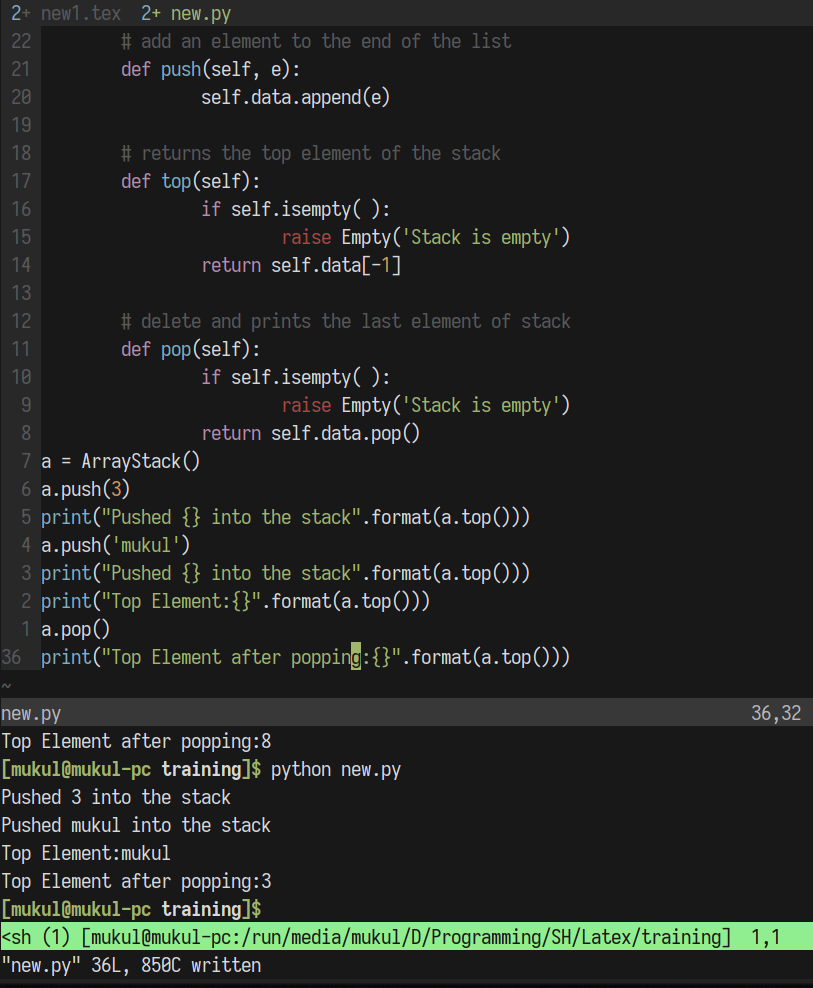
\includegraphics[scale=0.45]{fig3.png}
	\caption{\textsf{Output of listing 2.2}}
\end{figure}
\rule{15cm}{0.5mm}
\chapter{new}
\section{new1}
\end{document}
